\documentclass{article}
\usepackage{graphicx}
\begin{document}
\pagenumbering{gobble}
\vfill
\begin{center}
    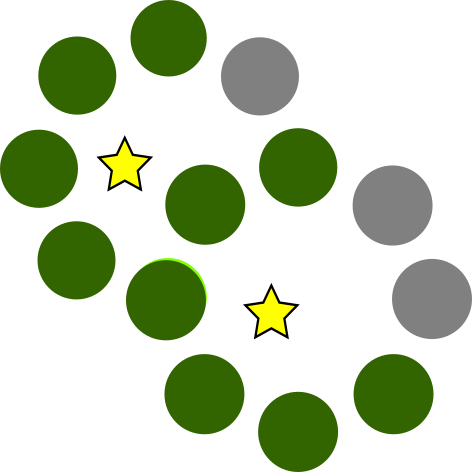
\includegraphics[scale=0.12]{../img/favicon.png}\\
{\huge Temporal Issue Tracking System\\}
{\Large User Manual}
\end{center}
\vfill
\newpage
\tableofcontents
\newpage
\setcounter{page}{3}
\pagenumbering{arabic}
\section{Logical model}
\includegraphics[width=\textwidth]{img/uml.png}
\section{Database}
Application utilizes MySQL database management system. All the database queries are executed as prepared statements in order to provide security. Credentials are stored in the form of username and password hash pair.
\section{PHP}
PHP code is split into several files. Header is implemented in \texttt{header.php}, database connection utilities are in \texttt{db.php}, rest of the files implement different pages of the application and are name accordingly.\\
Header is injected into each page and contains context actions specific for each page.\\
Passwords are hashed using the salt, combined from the password itself and additional characters, see \texttt{signup.php} or \texttt{login.php}.
\section{CSS}
CSS styles are stored in separate files, \texttt{style.css} being common for the entire application one and \texttt{header.css} is common for the part of the application, an authorized user can see. \texttt{footer.css} is a common footer for the list pages. The rest of the files correspond each to its own page and are named accordingly.\\
Pseudoelements are used to style placeholders.\\
Most elements' dimensions are tied to a font size so that application can be easily scaled.\\
\section{JavaScript}
JavaScript is utilezed for pre-validation of the form fields, but application if fully functional without it.\\
Script files are separated from the main code, each script corresponds to a page it's named after.
\end{document}
